\documentclass{article}%
\usepackage[T1]{fontenc}%
\usepackage[utf8]{inputenc}%
\usepackage{lmodern}%
\usepackage{textcomp}%
\usepackage{lastpage}%
\usepackage{parskip}%
\usepackage[top=4cm,hmargin=2cm,headheight=65pt,footskip=65pt]{geometry}%
\usepackage{amsmath}%
\usepackage{graphicx}%
\usepackage{needspace}%
\usepackage{color}%
\usepackage{longtable}%
\usepackage{multirow}%
\usepackage[table]{xcolor}%
\usepackage{fancyhdr}%
\usepackage{tabularx}%
%
\definecolor{OsdagGreen}{HTML}{D5DF93}%
\fancypagestyle{header}{ 
\renewcommand{\headrulewidth}{0pt}%
\renewcommand{\footrulewidth}{0pt}%
\fancyhead{ 
}%
\fancyfoot{ 
}%
\fancyhead[C]{ 
\begin{tabularx}{\textwidth}{|l|p{6cm}|l|X|}%
\hline%
\rowcolor{OsdagGreen}%
Company Name&&Project Title&\\%
\hline%
\rowcolor{OsdagGreen}%
Group/Team Name&&Subtitle&\\%
\hline%
\rowcolor{OsdagGreen}%
Designer&&Job Number&\\%
\hline%
\rowcolor{OsdagGreen}%
Date&09 /06 /2020&Client&\\%
\hline%
\end{tabularx}
}%
\fancyfoot[R]{ 
Page \thepage
}
}%
%
\begin{document}%
\normalsize%
\fontsize{8}{12}%
\selectfont%
\pagestyle{header}%
\section{Input Parameters}%
\label{sec:InputParameters}%
\renewcommand{\arraystretch}{1.2}%
\begin{longtable}{|p{5cm}|p{2cm}|p{2cm}|p{2cm}|p{5cm}|}%
\hline%
\hline%
\multicolumn{3}{|c|}{Module}&\multicolumn{2}{|c|}{Tension Members Bolted Design}\\%
\hline%
\hline%
\multicolumn{3}{|c|}{Axial (kN) *}&\multicolumn{2}{|c|}{500.0}\\%
\hline%
\hline%
\multicolumn{3}{|c|}{Length (mm) *}&\multicolumn{2}{|c|}{5000.0}\\%
\hline%
\hline%
\multicolumn{3}{|c|}{Section Size*}&\multicolumn{2}{|c|}{Ref List of Input Section}\\%
\hline%
\hline%
\multicolumn{5}{|c|}{\textbf{Bolt Details}}\\%
\hline%
\multicolumn{3}{|c|}{\multirow{2}{*}{Diameter (mm)*}}&\multicolumn{2}{|c|}{{[}12.0, 16.0, 20.0, 24.0, 30.0, }\\%
\multicolumn{3}{|c|}{\multirow{2}{*}{}}&\multicolumn{2}{|c|}{36.0{]}}\\%
\hline%
\multicolumn{3}{|c|}{\multirow{2}{*}{Grade *}}&\multicolumn{2}{|c|}{{[}3.6, 4.6, 4.8, 5.6, 5.8, 6.8, }\\%
\multicolumn{3}{|c|}{\multirow{2}{*}{}}&\multicolumn{2}{|c|}{8.8, 9.8, 10.9, 12.9{]}}\\%
\hline%
\hline%
\multicolumn{3}{|c|}{Type *}&\multicolumn{2}{|c|}{Bearing Bolt}\\%
\hline%
\hline%
\multicolumn{3}{|c|}{Bolt hole type}&\multicolumn{2}{|c|}{Standard}\\%
\hline%
\hline%
\multicolumn{3}{|c|}{Type of edges}&\multicolumn{2}{|c|}{a {-} Sheared or hand flame cut}\\%
\hline%
\hline%
\multicolumn{3}{|c|}{Are the members exposed to corrosive influences}&\multicolumn{2}{|c|}{False}\\%
\hline%
\hline%
\multicolumn{5}{|c|}{\textbf{Plate Details}}\\%
\hline%
\multicolumn{3}{|c|}{\multirow{5}{*}{Plate Thickness (mm)*}}&\multicolumn{2}{|c|}{{[}3.0, 4.0, 5.0, 6.0, 8.0, 10.0,}\\%
\multicolumn{3}{|c|}{\multirow{5}{*}{}}&\multicolumn{2}{|c|}{ 12.0, 14.0, 16.0, 18.0, 20.0,}\\%
\multicolumn{3}{|c|}{\multirow{5}{*}{}}&\multicolumn{2}{|c|}{ 22.0, 24.0, 25.0, 26.0, 28.0,}\\%
\multicolumn{3}{|c|}{\multirow{5}{*}{}}&\multicolumn{2}{|c|}{ 30.0, 32.0, 36.0, 40.0, 45.0,}\\%
\multicolumn{3}{|c|}{\multirow{5}{*}{}}&\multicolumn{2}{|c|}{ 50.0, 56.0, 63.0, 80.0{]}}\\%
\hline%
\hline%
\multicolumn{3}{|c|}{Material *}&\multicolumn{2}{|c|}{E 250 (Fe 410 W)A}\\%
\hline%
\hline%
\multicolumn{3}{|c|}{Ultimate strength, fu (MPa)}&\multicolumn{2}{|c|}{410}\\%
\hline%
\hline%
\multicolumn{3}{|c|}{Yield Strength , fy (MPa)}&\multicolumn{2}{|c|}{250}\\%
\hline%
\hline%
\multicolumn{5}{|c|}{\textbf{Safety Factors {-} IS 800:2007 Table 5 (Clause 5.4.1) }}\\%
\hline%
\hline%
\multicolumn{3}{|c|}{Governed by Yielding}&\multicolumn{2}{|c|}{$\begin{aligned}\gamma_{m0}&=1.1\end{aligned}$}\\%
\hline%
\hline%
\multicolumn{3}{|c|}{Governed by Ultimate Stress}&\multicolumn{2}{|c|}{$\begin{aligned}\gamma_{m1}&=1.25\end{aligned}$}\\%
\hline%
\hline%
\multicolumn{3}{|c|}{Connection Bolts {-} Bearing Type}&\multicolumn{2}{|c|}{$\begin{aligned}\gamma_{mb}&=1.25\end{aligned}$}\\%
\hline%
\end{longtable}%
\subsection{List of Input Section}%
\label{subsec:ListofInputSection}%
\renewcommand{\arraystretch}{1.2}%
\begin{longtable}{|p{8cm}|p{8cm}|}%
\hline%
\multicolumn{1}{|c|}{Section Size*}&\multicolumn{1}{|c|}{{[}'20 x 20 x 3', '20 x 20 x 4', '25 x 25 x 3', '25 x 25 x 4', '25 x 25 x 5', '30 x 30}\\%
\hline%
\hline%
\multicolumn{1}{|c|}{ }&\multicolumn{1}{|c|}{ x 3', '30 x 30 x 4', '30 x 30 x 5', '35 x 35 x 3', '35 x 35 x 4', '35 x 35 x 5', '}\\%
\hline%
\hline%
\multicolumn{1}{|c|}{ }&\multicolumn{1}{|c|}{35 x 35 x 6', '40 x 40 x 3', '40 x 40 x 4', '40 x 40 x 5', '40 x 40 x 6', '45 x 45 }\\%
\hline%
\hline%
\multicolumn{1}{|c|}{ }&\multicolumn{1}{|c|}{x 3', '45 x 45 x 4', '45 x 45 x 5', '45 x 45 x 6', '50 x 50 x 3', '50 x 50 x 4', '5}\\%
\hline%
\hline%
\multicolumn{1}{|c|}{ }&\multicolumn{1}{|c|}{0 x 50 x 5', '50 x 50 x 6', '55 x 55 x 4', '55 x 55 x 5', '55 x 55 x 6', '55 x 55 x}\\%
\hline%
\hline%
\multicolumn{1}{|c|}{ }&\multicolumn{1}{|c|}{ 8', '60 x 60 x 4', '60 x 60 x 5', '60 x 60 x 6', '60 x 60 x 8', '65 x 65 x 4', '65}\\%
\hline%
\hline%
\multicolumn{1}{|c|}{ }&\multicolumn{1}{|c|}{ x 65 x 5', '65 x 65 x 6', '65 x 65 x 8', '70 x 70 x 5', '70 x 70 x 6', '70 x 70 x }\\%
\hline%
\hline%
\multicolumn{1}{|c|}{ }&\multicolumn{1}{|c|}{8', '70 x 70 x 10', '75 x 75 x 5', '75 x 75 x 6', '75 x 75 x 8', '75 x 75 x 10', '8}\\%
\hline%
\hline%
\multicolumn{1}{|c|}{ }&\multicolumn{1}{|c|}{0 x 80 x 6', '80 x 80 x 8', '80 x 80 x 10', '80 x 80 x 12', '90 x 90 x 6', '90 x 90}\\%
\hline%
\hline%
\multicolumn{1}{|c|}{ }&\multicolumn{1}{|c|}{ x 8', '90 x 90 x 10', '90 x 90 x 12', '100 x 100 x 6', '100 x 100 x 8', '100 x 100}\\%
\hline%
\hline%
\multicolumn{1}{|c|}{ }&\multicolumn{1}{|c|}{ x 10', '100 x 100 x 12', '110 x 110 x 8', '110 x 110 x 10', '110 x 110 x 12', '110}\\%
\hline%
\hline%
\multicolumn{1}{|c|}{ }&\multicolumn{1}{|c|}{ x 110 x 16', '130 x 130 x 8', '130 x130 x 10', '130 x130 x 12', '130 x130 x 16', '}\\%
\hline%
\hline%
\multicolumn{1}{|c|}{ }&\multicolumn{1}{|c|}{150 x 150 x 10', '150 x 150 x 12', '150 x 150 x 16', '150 x 150 x 20', '200 x 200 x}\\%
\hline%
\hline%
\multicolumn{1}{|c|}{ }&\multicolumn{1}{|c|}{ 12', '200 x 200 x 16', '200 x 200 x 20', '200 x 200 x 25', '50 x 50 x 7', '50 x 50}\\%
\hline%
\hline%
\multicolumn{1}{|c|}{ }&\multicolumn{1}{|c|}{ x 8', '55 x 55 x 10', '60 x 60 x 10', '65 x 65 x 10', '70 x 70 x 7', '100 x 100 x }\\%
\hline%
\hline%
\multicolumn{1}{|c|}{ }&\multicolumn{1}{|c|}{7', '100 x 100 x 15', '120 x 120 x 8', '120 x 120 x 10', '120 x 120 x 12', '120 x 1}\\%
\hline%
\hline%
\multicolumn{1}{|c|}{ }&\multicolumn{1}{|c|}{20 x 15', '130 x 130 x 9', '150 x 150 x 15', '150 x 150 x 18', '180 x 180 x 15', '1}\\%
\hline%
\hline%
\multicolumn{1}{|c|}{ }&\multicolumn{1}{|c|}{80 x 180 x 18', '180 x 180 x 20', '200 x 200 x 24', '30 x 20 x 3', '30 x 20 x 4', '}\\%
\hline%
\hline%
\multicolumn{1}{|c|}{ }&\multicolumn{1}{|c|}{30 x 20 x 5', '40 x 25 x 3', '40 x 25 x 4', '40 x 25 x 5', '40 x 25 x 6', '45 x 30 }\\%
\hline%
\hline%
\multicolumn{1}{|c|}{ }&\multicolumn{1}{|c|}{x 3', '45 x 30 x 4', '45 x 30 x 5', '45 x 30 x 6', '50 x 30 x 3', '50 x 30 x 4', '5}\\%
\hline%
\hline%
\multicolumn{1}{|c|}{ }&\multicolumn{1}{|c|}{0 x 30 x 5', '50 x 30 x 6', '60 x 40 x 5', '60 x 40 x 6', '60 x 40 x 8', '65 x 45 x}\\%
\hline%
\hline%
\multicolumn{1}{|c|}{ }&\multicolumn{1}{|c|}{ 5', '65 x 45 x 6', '65 x 45 x 8', '70 x 45 x 5', '70 x 45 x 6', '70 x 45 x 8', '70}\\%
\hline%
\hline%
\multicolumn{1}{|c|}{ }&\multicolumn{1}{|c|}{ x 45 x 10', '75 x 50 x 5', '75 x 50 x 6', '75 x 50 x 8', '75 x 50 x 10', '80 x 50 }\\%
\hline%
\hline%
\multicolumn{1}{|c|}{ }&\multicolumn{1}{|c|}{x 5', '80 x 50 x 6', '80 x 50 x 8', '80 x 50 x 10', '90 x 60 x 6', '90 x 60 x 8', '}\\%
\hline%
\hline%
\multicolumn{1}{|c|}{ }&\multicolumn{1}{|c|}{90 x 60 x 10', '90 x 60 x 12', '100 x 65 x 6', '100 x 65 x 8', '100 x 65 x 10', '10}\\%
\hline%
\hline%
\multicolumn{1}{|c|}{ }&\multicolumn{1}{|c|}{0 x 75 x 6', '100 x 75 x 8', '100 x 75 x 10', '100 x 75 x 12', '125 x 75 x 6', '125}\\%
\hline%
\hline%
\multicolumn{1}{|c|}{ }&\multicolumn{1}{|c|}{ x 75 x 8', '125 x 75 x 10', '125 x 95 x 6', '125 x 95 x 8', '125 x 95 x 10', '125 }\\%
\hline%
\hline%
\multicolumn{1}{|c|}{ }&\multicolumn{1}{|c|}{x 95 x 12', '150 x 115 x 8', '150 x 115 x 10', '150 x 115 x 12', '150 x 115 x 16', }\\%
\hline%
\hline%
\multicolumn{1}{|c|}{ }&\multicolumn{1}{|c|}{'200 x 100 x 10', '200 x 100 x 12', '200 x 100 x 16', '200 x 150 x 10', '200 x 150 }\\%
\hline%
\hline%
\multicolumn{1}{|c|}{ }&\multicolumn{1}{|c|}{x 12', '200 x 150 x 16', '200 x 150 x 20', '40 x 20 x 3', '40 x 20 x 4', '40 x 20 x}\\%
\hline%
\hline%
\multicolumn{1}{|c|}{ }&\multicolumn{1}{|c|}{ 5', '60 x 30 x 5', '60 x 30 x 6', '60 x 40 x 7', '65 x 50 x 5', '65 x 50 x 6', '65}\\%
\hline%
\hline%
\multicolumn{1}{|c|}{ }&\multicolumn{1}{|c|}{ x 50 x 7', '65 x 50 x 8', '70 x 50 x 5', '70 x 50 x 6', '70 x 50 x 7', '70 x 50 x }\\%
\hline%
\hline%
\multicolumn{1}{|c|}{ }&\multicolumn{1}{|c|}{8', '75 x 50 x 7', '80 x 40 x 5', '80 x 40 x 6', '80 x 40 x 7', '80 x 40 x 8', '80 }\\%
\hline%
\hline%
\multicolumn{1}{|c|}{ }&\multicolumn{1}{|c|}{x 60 x 6', '80 x 60 x 7', '80 x 60 x 8', '90 x 65 x 6', '90 x 65 x 7', '90 x 65 x 8}\\%
\hline%
\hline%
\multicolumn{1}{|c|}{ }&\multicolumn{1}{|c|}{', '90 x 65 x 10', '100 x 50 x 6', '100 x 50 x 7', '100 x 50 x 8', '100 x 50 x 10',}\\%
\hline%
\hline%
\multicolumn{1}{|c|}{ }&\multicolumn{1}{|c|}{ '100 x 65 x 7', '120 x 80 x 8', '120 x 80 x 10', '120 x 80 x 12', '125 x 75 x 12',}\\%
\hline%
\hline%
\multicolumn{1}{|c|}{ }&\multicolumn{1}{|c|}{ '135 x 65 x 8', '135 x 65 x 10', '135 x 65 x 12', '150 x 75 x 9', '150 x 75 x 15',}\\%
\hline%
\hline%
\multicolumn{1}{|c|}{ }&\multicolumn{1}{|c|}{ '150 x 90 x 10', '150 x 90 x 12', '150 x 90 x 15', '200 x 100 x 15', '200 x 150 x }\\%
\hline%
\hline%
\multicolumn{1}{|c|}{ }&\multicolumn{1}{|c|}{15', '200 x 150 x 18'{]}}\\%
\hline%
\end{longtable}

%
\Needspace{10\baselineskip}%
\newpage%
\section{Design Checks}%
\label{sec:DesignChecks}%
\subsection{Selected Member Data}%
\label{subsec:SelectedMemberData}%
\renewcommand{\arraystretch}{1.2}%
\begin{longtable}{|p{5cm}|p{2cm}|p{2cm}|p{2cm}|p{5cm}|}%
\hline%
\hline%
\multirow{15}{*}{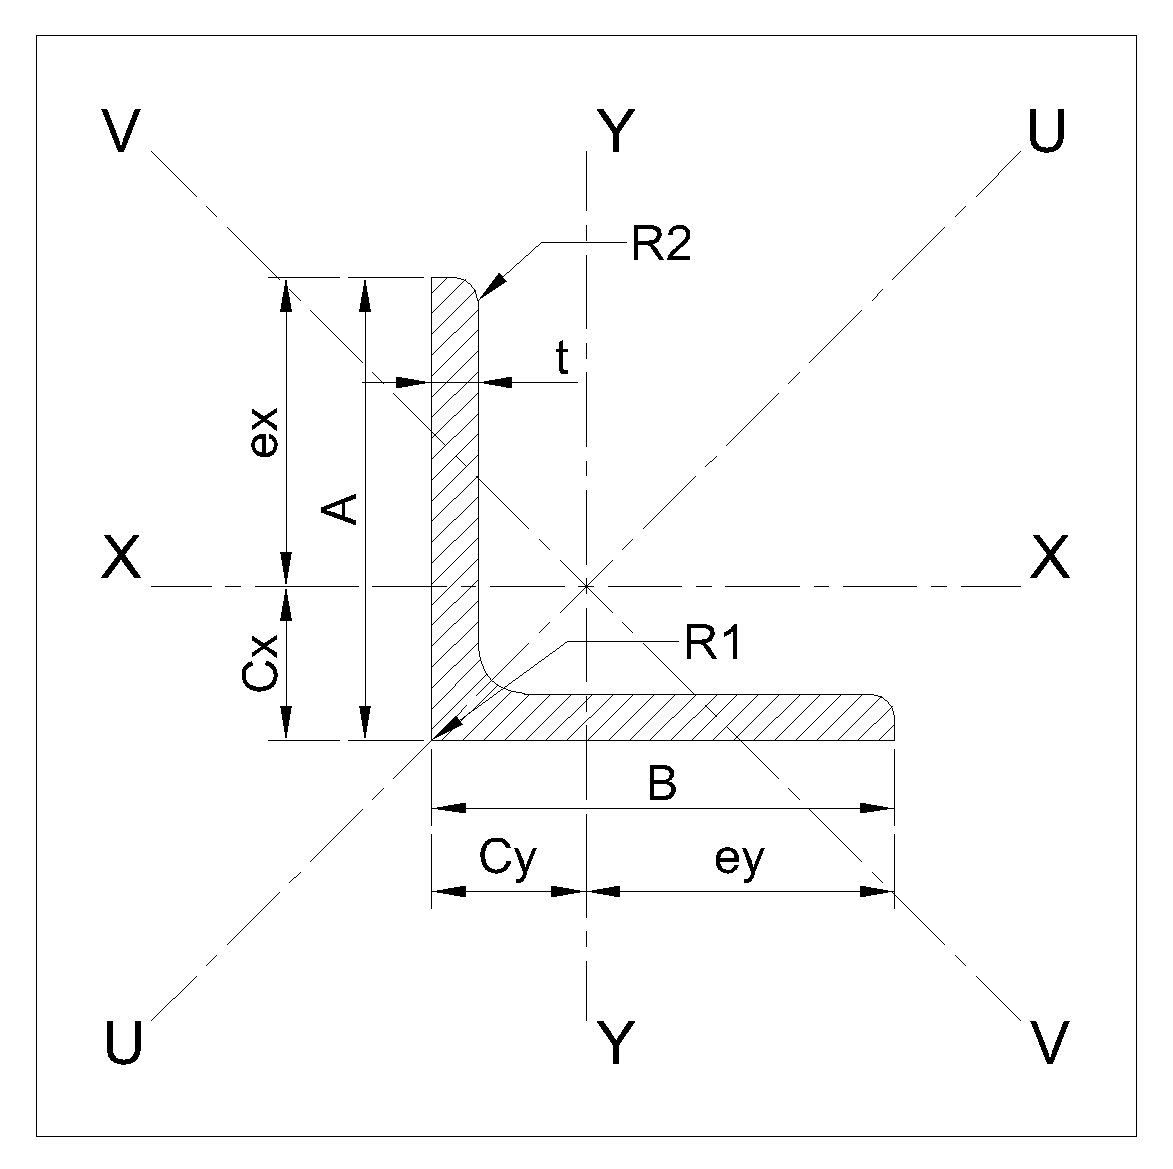
\includegraphics[width=5cm,height=5cm]{E:/workspace/Osdag3/ResourceFiles/images/Equal.png}}&\multicolumn{2}{|c|}{Section Size*}&\multicolumn{2}{|c|}{('100 x 100 x 12', 'Angles')}\\%
\cline{2%
-%
5}%
&\multicolumn{2}{|c|}{Material *}&\multicolumn{2}{|c|}{E 250 (Fe 410 W)A}\\%
\cline{2%
-%
5}%
&\multicolumn{2}{|c|}{Ultimate strength, fu (MPa)}&\multicolumn{2}{|c|}{410}\\%
\cline{2%
-%
5}%
&\multicolumn{2}{|c|}{Yield Strength , fy (MPa)}&\multicolumn{2}{|c|}{250}\\%
\cline{2%
-%
5}%
&Mass&17.83&Iu(mm4)&3330000.0\\%
\cline{2%
-%
5}%
&Area(mm2) {-} A&2270.0&Iv(mm4)&872000.0\\%
\cline{2%
-%
5}%
&a(mm)&100.0&rz(mm)&30.4\\%
\cline{2%
-%
5}%
&b(mm)&100.0&ry(mm)&30.4\\%
\cline{2%
-%
5}%
&t(mm)&12.0&ru(mm)&38.3\\%
\cline{2%
-%
5}%
&R1(mm)&8.5&rv(mm)&19.6\\%
\cline{2%
-%
5}%
&R2(mm)&0.0&Zz(mm3)&29800.0\\%
\cline{2%
-%
5}%
&Cy(mm)&29.3&Zy(mm3)&29800.0\\%
\cline{2%
-%
5}%
&Cz(mm)&29.3&Zpz(mm3)&53600.0\\%
\cline{2%
-%
5}%
&Iz(mm4)&2100000.0&Zpy(mm3)&29800.0\\%
\cline{2%
-%
5}%
&Iy(mm4)&2100000.0&r(mm)&19.6\\%
\cline{2%
-%
5}%
\hline%
\end{longtable}

%
\newpage%
\subsection{Spacing Checks}%
\label{subsec:SpacingChecks}%
\renewcommand{\arraystretch}{1.2}%
\begin{longtable}{|p{2.5cm}|p{7.5cm}|p{3cm}|p{3cm}|}%
\hline%
\rowcolor{OsdagGreen}%
Check&Required&Provided&Remarks\\%
\hline%
\endhead%
\hline%
Min.Diameter (mm)&&$\begin{aligned} d &=16\end{aligned}$&\\%
\hline%
Hole Diameter (mm)& &$\begin{aligned} d_0 &=18\end{aligned}$&\\%
\hline%
Min. Gauge (mm)&$\begin{aligned}p/g_{min}&= 2.5 ~ d&\\ =&2.5*16.0&=40.0\end{aligned}$&40&Row Limit (rl) = 1\\%
\hline%
Min. Edge Distance (mm)&$\begin{aligned}e/e`_{min} &=[1.5~or~ 1.7] * d_0\\ &=1.7*18.0=30.6 \end{aligned}$&35&\\%
\hline%
Spacing Check&$\begin{aligned} depth & = 2 * e + (r_l -1) * g\\ & = 2 * 35+(1-1)*40\\ & = 70\end{aligned}$&79.5&Pass\\%
\hline%
\end{longtable}

%
\newpage%
\subsection{Member Checks}%
\label{subsec:MemberChecks}%
\renewcommand{\arraystretch}{1.2}%
\begin{longtable}{|p{2.5cm}|p{4.5cm}|p{8cm}|p{1cm}|}%
\hline%
\rowcolor{OsdagGreen}%
Check&Required&Provided&Remarks\\%
\hline%
\endhead%
\hline%
Tension Yielding Capacity (kN)&&$\begin{aligned}T_{dg}~or~A_c&= \frac{1 * A_g ~ f_y}{\gamma_{m0}}\\ &= \frac{1*2270.0*250}{1.1}\\ &= 515.91\end{aligned}$&\\%
\hline%
Tension Rupture Capacity (kN)&&$\begin{aligned}\beta &= 1.4 - 0.076*\frac{w}{t}*\frac{f_{y}}{0.9*f_{u}}*\frac{b_s}{L_c}\\ &\leq\frac{0.9*f_{u}*\gamma_{m0}}{f_{y}*\gamma_{m1}} \geq 0.7 \\ &= 1.4 - 0.076*\frac{100.0}{12.0}*\frac{250}{0.9*410}*\frac{148.25}{315 }\\ &\leq\frac{0.9* 410*1.1}{250*1.25} \geq 0.7 \\ &= 1.2\\ T_{dn} &= 1*(\frac{0.9*A_{nc}*f_{u}}{\gamma_{m1}} + \frac{\beta * A_{go} * f_{y}}{\gamma_{m0}})\\ &= 1*(\frac{0.9* 840.0*410}{1.25} + \frac{1.2*1200.0*250}{1.1})\\ &= 575.24\end{aligned}$&\\%
\hline%
Block Shear Capacity (kN)&&$\begin{aligned}T_{db1} &= \frac{A_{vg} f_{y}}{\sqrt{3} \gamma_{m0}} + \frac{0.9 A_{tn} f_{u}}{\gamma_{m1}}\\ T_{db2} &= \frac{0.9*A_{vn} f_{u}}{\sqrt{3} \gamma_{m1}} + \frac{A_{tg} f_{y}}{\gamma_{m0}}\\ T_{db} &= min(T_{db1}, T_{db2})= 548.13\end{aligned}$&\\%
\hline%
Tension Capacity (kN)&500.0&$\begin{aligned} T_d &= min(T_{dg},T_{dn},T_{db})\\ &= min(515.91,575.24,548.13)\\ &=515.91\end{aligned}$&Pass\\%
\hline%
Slenderness&$\begin{aligned}\frac{K * L}{r} &\leq 400\end{aligned}$&$\begin{aligned}\frac{K * L}{r} &= \frac{1*5000.0}{19.6}\\ &= 255.1\end{aligned}$&Pass\\%
\hline%
Utilization Ratio&$\begin{aligned} Utilization~Ratio &\leq 1 \end{aligned}$&$\begin{aligned} Utilization~Ratio &= \frac{F}{Td}&=\frac{500.0}{515.91}\\ &= 0.97\end{aligned}$&\\%
\hline%
Axial Load Considered (kN)&$\begin{aligned} Ac_{min} &= 0.3 * A_c\\ &= 0.3 *515.91\\ &=154.77\\ Ac_{max} &=515.91\end{aligned}$&$\begin{aligned} A &=500.0\end{aligned}$&Pass\\%
\hline%
\end{longtable}

%
\newpage%
\subsection{Bolt Checks}%
\label{subsec:BoltChecks}%
\renewcommand{\arraystretch}{1.2}%
\begin{longtable}{|p{2.5cm}|p{5.5cm}|p{7cm}|p{1cm}|}%
\hline%
\rowcolor{OsdagGreen}%
Check&Required&Provided&Remarks\\%
\hline%
\endhead%
\hline%
Diameter (mm)&Bolt Quantity Optimisation&$\begin{aligned} d &=16\end{aligned}$&\\%
\hline%
Hole Diameter (mm)& &$\begin{aligned} d_0 &=18\end{aligned}$&\\%
\hline%
Grade&Bolt Grade Optimisation&10.9&\\%
\hline%
Bolt Ultimate Strength (N/mm2)&&$\begin{aligned} f_{ub} &=1040.0\end{aligned}$&\\%
\hline%
Bolt Yield Strength (N/mm2)&&$\begin{aligned} f_{yb} &=940.0\end{aligned}$&\\%
\hline%
Nominal Stress Area (mm2)& &$\begin{aligned} A_{nb} &=157~( Ref~IS~1367-3~(2002))\end{aligned}$&\\%
\hline%
Min. Pitch (mm)&$\begin{aligned}p/g_{min}&= 2.5 ~ d&\\ =&2.5*16.0&=40.0\end{aligned}$&45&Pass\\%
\hline%
Max. Pitch (mm)&$\begin{aligned}p/g_{max} &=\min(32~t,~300~mm)&\\ &=\min(32 *~12.0,~ 300 ~mm)\\&=300\\  t& = min(24.0,24.0)\end{aligned}$&45&Pass\\%
\hline%
Min. Gauge (mm)&$\begin{aligned}p/g_{min}&= 2.5 ~ d&\\ =&2.5*16.0&=40.0\end{aligned}$&0&N/A\\%
\hline%
Max. Gauge (mm)&$\begin{aligned}p/g_{max} &=\min(32~t,~300~mm)&\\ &=\min(32 *~12.0,~ 300 ~mm)\\&=300\\  t& = min(24.0,24.0)\end{aligned}$&0&N/A\\%
\hline%
Min. End Distance (mm)&$\begin{aligned}e/e`_{min} &=[1.5~or~ 1.7] * d_0\\ &=1.7*18.0=30.6 \end{aligned}$&35&Pass\\%
\hline%
Max. End Distance (mm)&$\begin{aligned}e/e`_{max} &= 12~ t~ \varepsilon&\\ \varepsilon &= \sqrt{\frac{250}{f_y}}\\ e/e`_{max}&=12 ~*12.0*\sqrt{\frac{250}{250}}\\ &=144.0\\ \end{aligned}$&35&Pass\\%
\hline%
Min. Edge Distance (mm)&$\begin{aligned}e/e`_{min} &=[1.5~or~ 1.7] * d_0\\ &=1.7*18.0=30.6 \end{aligned}$&39.75&Pass\\%
\hline%
Max. Edge Distance (mm)&$\begin{aligned}e/e`_{max} &= 12~ t~ \varepsilon&\\ \varepsilon &= \sqrt{\frac{250}{f_y}}\\ e/e`_{max}&=12 ~*12.0*\sqrt{\frac{250}{250}}\\ &=144.0\\ \end{aligned}$&39.75&Pass\\%
\hline%
Kb& &$\begin{aligned} k_b & = min(\frac{e}{3*d_0},\frac{p}{3*d_0}-0.25,\frac{f_{ub}}{f_u},1.0)\\ & = min(\frac{35}{3*18.0},\frac{45}{3*18.0}-0.25,\frac{1040.0}{410},1.0)\\ & = min(0.65,0.58,2.54,1.0)\\ & = 0.58\end{aligned}$&\\%
\hline%
Shear Capacity (kN)&&$\begin{aligned}V_{dsb} &= \frac{f_{ub} ~n_n~ A_{nb}}{\sqrt{3} ~\gamma_{mb}}\\ &= \frac{1040.0*1*157}{\sqrt{3}~*~1.25}\\ &= 75.42\end{aligned}$&\\%
\hline%
Bearing Capacity (kN)&&$\begin{aligned}V_{dpb} &= \frac{2.5~ k_b~ d~ t~ f_u}{\gamma_{mb}}\\ &= \frac{2.5~*0.58*16.0*12.0*410}{1.25}\\ &=91.32\end{aligned}$&\\%
\hline%
Capacity (kN)&&$\begin{aligned}V_{db} &= min~ (V_{dsb}, V_{dpb})\\ &= min~ (75.42,91.32)\\ &=75.42\end{aligned}$&\\%
\hline%
No of Bolts&$\begin{aligned}R_{u} &= \sqrt{V_u^2+A_u^2}\\ n_{trial} &= R_u/ V_{bolt}\\ R_{u} &= \frac{\sqrt{0.0^2+500.0^2}}{75.42}\\ &=7\end{aligned}$&$\begin{aligned} n &=8\end{aligned}$&\\%
\hline%
No of Columns&&$\begin{aligned} n_c &=8\end{aligned}$&\\%
\hline%
No of Rows&&$\begin{aligned} n_r &=1\end{aligned}$&\\%
\hline%
Bolt Capacity post Long Joint (kN)&$\begin{aligned} &if~l\geq 15 * d~then~V_{rd} = \beta_{ij} * V_{db} \\ & if~l < 15 * d~then~V_{rd} = V_{db} \\ & where,\\ & l = ((nc~or~nr) - 1) * (p~or~g) \\ & \beta_{ij} = 1.075 - l/(200 * d) \\ & but~0.75\leq\beta_{ij}\leq1.0 \end{aligned}$&$\begin{aligned} l&= ((nc~or~nr) - 1) * (p~or~g) \\  &= (8 - 1) * 45=315\\  &= (1 - 1) * 0=0\\  l&= 315\\ & 15 * d = 15 * 16.0 = 240.0 \\ & since,~l \geq 15 * d~then~V_{rd} = \beta_{ij} * V_{db} \\ & \beta_{ij} = 1.075 - 315/(200*16.0) =0.98\\ & V_{rd} = 0.98 * 75.42=73.91 \end{aligned}$&\\%
\hline%
Capacity (kN)&62.5&73.91&Pass\\%
\hline%
\end{longtable}

%
\newpage%
\subsection{Gusset Plate Checks}%
\label{subsec:GussetPlateChecks}%
\renewcommand{\arraystretch}{1.2}%
\begin{longtable}{|p{2.5cm}|p{5cm}|p{7.5cm}|p{1cm}|}%
\hline%
\rowcolor{OsdagGreen}%
Check&Required&Provided&Remarks\\%
\hline%
\endhead%
\hline%
Min.Height (mm)&&$\begin{aligned} H &= 1* Depth + clearance \\ &=(1*100.0)+30.0\\ &= 130\end{aligned}$&\\%
\hline%
Min.Length (mm)&5000.0&$\begin{aligned} L &= (nc -1) * p + 2 * e\\ &= (8-1) *45+ (2 *35)\\ &= 385\end{aligned}$&Pass\\%
\hline%
Thickness (mm)&&$\begin{aligned} t_p &=24.0\end{aligned}$&\\%
\hline%
Tension Yielding Capacity (kN)&&$\begin{aligned} T_{dg} &= \frac{l*t*f_y}{\gamma_{mo}}\\ &=\frac{1*100.0*24.0*250}{1.1}\\ &=545.45\end{aligned}$&\\%
\hline%
Tension Rupture Capacity (kN)&&$\begin{aligned} T_{dn} &= \frac{0.9*A_{n}*f_u}{\gamma_{m1}}\\ &=\frac{1*0.9* (100.0-1*18.0)*24.0*410}{1.25}\\ &=580.95\end{aligned}$&\\%
\hline%
Block Shear Capacity (kN)&&$\begin{aligned}T_{db1} &= \frac{A_{vg} f_{y}}{\sqrt{3} \gamma_{m0}} + \frac{0.9 A_{tn} f_{u}}{\gamma_{m1}}\\ T_{db2} &= \frac{0.9*A_{vn} f_{u}}{\sqrt{3} \gamma_{m1}} + \frac{A_{tg} f_{y}}{\gamma_{m0}}\\ T_{db} &= min(T_{db1}, T_{db2})= 1096.26\end{aligned}$&\\%
\hline%
Tension Capacity (kN)&$\begin{aligned} A &=500.0\end{aligned}$&$\begin{aligned} T_d &= min(T_{dg},T_{dn},T_{db})\\ &= min(545.45,580.95,1096.26)\\ &=545.45\end{aligned}$&Pass\\%
\hline%
\end{longtable}

%
\Needspace{10\baselineskip}%
\newpage%
\section{3D View}%
\label{sec:3DView}%


\begin{figure}[h!]%
\centering%
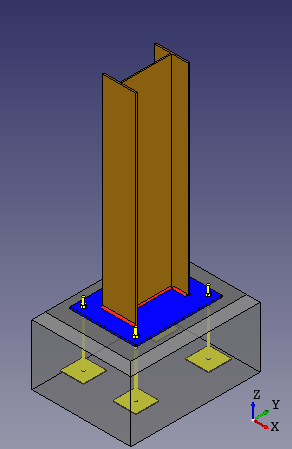
\includegraphics[width=\linewidth]{E:/workspace/Osdag3/ResourceFiles/images/3d.png}%
\caption{3D View}%
\end{figure}

%
\end{document}